\chapter{面对客流剧烈变化的迭代学习模型预测控制方法}\label{chap:05}

\setcounter{algorithm}{0} % 重置算法计数器

\section{问题描述}
\label{section2}

在构建状态空间模型之前，首先对所研究的交通场景进行描述。基于列车实际运行过程，提出其动态方程，为后续建模奠定基础。

\subsection{城际高速铁路的运行场景}

为建立有效的城际高速铁路线路状态空间模型并设计实时控制器，需对列车运行场景进行数学刻画，并对运行过程进行动态分析。

考虑一条连接城市 A 与 B 的双线城际高速铁路线路，沿线共设 $N$ 个车站，有 $M$ 列列车（$M > N$）在线路上循环运行。所有列车均在每一站停靠，供乘客上下车。当列车抵达某一端点城市后，立即折返继续驶向另一端点城市。由于城际高速铁路采用类似城市轨道交通的高密度公交化运营模式，不考虑列车越行或交会操作；同时，所有列车均实行站站停模式，即不采用小交路运行或跳站策略。

在城际高速铁路中，站间距通常较长，在高峰时段常出现多列车（$M > N$）同时在线运行的情形 \cite{Kang2024}。此外，为保障各站乘客的服务水平，线路普遍采用全站停靠的运行模式 \cite{Han2021}。另一方面，由于列车运行速度较为接近，越行需求较低；且越行操作需依赖特定基础设施（如越行线或双岛式站台），而此类设施在类地铁化运营的城际铁路中并不常见。因此，忽略越行操作符合当前城际高速铁路的实际运营实践 \cite{Gupta2016}。

本文所考虑的场景包含列车折返操作。目前，城际高速列车主要有两种折返方式：站前折返与尾端折返。对于站前折返，上下客与折返作业均在同一车站完成，可将其简化为单个车站建模；而对于尾端折返，则先在一个车站完成乘客下车，再于相邻车站完成上客，因此可建模为两个连续车站，其间运行时间即为折返耗时。综上，两类折返场景均可统一纳入一个包含 $M$ 列列车与 $N$ 个车站的通用模型中。

基于上述分析，本文将线路结构简化为**环形线路**（Loop Line），其定义如下：

\textbf{环形线路}：指由 $N$ 个车站（编号为 $1$ 至 $N$）组成的闭合线路，其中车站 $N$ 与车站 $1$ 相连，且一组列车（编号为 $1$ 至 $M$）按固定周期循环运行。所有列车在各站的发车顺序保持一致。任意一列列车依次停靠各站的顺序为：
\begin{equation*}
	\{1,2, \cdots, M, 1,2, \cdots, M, 1,2, \cdots\}
\end{equation*}
相应地，车站的访问序列为：
\begin{equation*}
	\{1,2, \cdots, N, 1,2, \cdots, N, 1,2, \cdots\}
\end{equation*}

由于该高速铁路线路具有环形结构，某列车在车站 $1$ 的状态变量在名义上与其前一站（即车站 $N$）的状态相关，并受历史交通状况演化的影响。

综上所述，实际的城际高速铁路线路可被抽象为一个包含 $N$ 个车站的环形模型。在此基础上，通过耦合交通动态与客流因素，建立列车运行的动态方程，并据此构建相应的状态空间模型。用于描述列车运行过程的关键变量如表~\ref{table1} 所示。

\begin{table}
	\centering
	\caption{变量及其定义}
	\label{table1}
	\begin{tabular}{cp{0.7\linewidth}}
		\hline
		变量 & 定义 \\
		\hline
		$t_{j}^{i}$ & 列车 $i$ 在车站 $j$ 的实际发车时刻 \\
		$r_{j}^{i}$ & 列车 $i$ 从车站 $j$ 到车站 $j+1$ 的实际运行时间 \\
		$s_{j}^{i}$ & 列车 $i$ 在车站 $j$ 的实际停站时间 \\
		$R_{j}$ & 车站 $j$ 到 $j+1$ 的图定运行时间 \\
		$u_{j}^{i}$ & 对列车 $i$ 在区间 $[j, j+1]$ 运行时间施加的重调度控制量 \\
		$T_{j}^{i}$ & 列车 $i$ 在车站 $j$ 的图定发车时刻 \\
		${w_1}_{j}^{i}$ & 运行时间的扰动项 \\
		${w_2}_{j}^{i}$ & 停站时间的扰动项 \\
		$w_{j}^{i}$ & 总扰动项（${w_1}_{j}^{i} + {w_2}_{j+1}^{i}$）\\
		$H$ & 相邻列车之间的标称发车间隔 \\
		$c_{j}$ & 车站 $j$ 的延误率，反映相邻列车发车间隔对停站时间的影响 \\
		$S$ & 最小停站时间 \\
		$x_{j}^{i}$ & 实际发车时刻 $t_j^i$ 相对于图定时刻 $T_j^i$ 的偏差 \\
		\hline
	\end{tabular}
\end{table}

\noindent\textbf{符号说明}：除非另有说明，变量或参数的上标 $i$ 表示列车编号，下标 $j$ 表示车站编号。为体现城际高速铁路的周期性运行特性，列车编号 $i$ 和车站编号 $j$ 分别对总列车数 $M$ 和总车站数 $N$ 取模。依此约定，相邻两列车可记为 $i$ 与 $i+1$（其中 $1 \leq i \leq M$，且列车 $M$ 之后为列车 $1$）；相邻两车站可记为 $j$ 与 $j+1$（其中 $1 \leq j \leq N$，且车站 $N$ 之后为车站 $1$）。

\subsection{列车交通动态方程}

基于城际高速铁路的实际运行情况，列车 $i$ 在车站 $j+1$ 的发车时刻可表示为 \cite{VanBreusegem1991}：
\begin{equation}
   t_{j+1}^{i}=t_{j}^{i}+r_{j}^{i}+s_{j+1}^{i} 
\label{eq1}
\end{equation}
其中，$r_{j}^{i}$ 为列车 $i$ 从车站 $j$ 至 $j+1$ 的实际运行时间，$s_{j+1}^{i}$ 为其在车站 $j+1$ 的停站时间。

实际运行时间可进一步分解为：
\begin{equation}
   r_{j}^{i}=R_{j}+u_{j}^{i}+{w_1}_{j}^{i}
\label{eq2}
\end{equation}
其中，$R_{j}$ 为图定运行时间，$u_{j}^{i}$ 为施加的重调度控制量，${w_1}_{j}^{i}$ 为由天气、轨道状态或信号延迟等外部因素引起的运行时间不确定性。

目前，部分城际高速铁路（如广深城际、珠机城际）已采用“公交化”运营模式，乘客无需提前购票。在此模式下，车站停站时间受站台客流及相邻列车发车间隔影响 \cite{Kang2024}。因此，停站时间可建模为：
\begin{equation}
    s_{j+1}^{i}=S+c_{j+1} (t_{j+1}^{i}-t_{j+1}^{i-1})+{w_2}_{j+1}^{i}
\label{eq3}
\end{equation}
其中，$S$ 为最小停站时间，$c_{j+1}$ 为车站 $j+1$ 的延误率，反映相邻列车发车间隔对停站时间的影响：发车间隔越长，站台积压乘客越多，上下车时间可能越长 \cite{Li2016a, VanBreusegem1991}。${w_2}_{j+1}^{i}$ 为停站时间的干扰项，用于刻画站台拥堵、乘客到达不规律或突发上下车事件等不确定性。

将式~(\ref{eq2}) 与 (\ref{eq3}) 中的扰动项合并，定义总扰动为：
\begin{equation}
    w_{j}^{i}={w_1}_{j}^{i}+{w_2}_{j+1}^{i}
\label{eq4}
\end{equation}

将式~(\ref{eq2}) 和 (\ref{eq3}) 代入式~(\ref{eq1})，并利用式~(\ref{eq4}) 合并扰动项，可得：
\begin{equation}
    (1-c_{j+1})t_{j+1}^{i}=t_{j}^{i}-c_{j+1}t_{j+1}^{i-1}+S+R_{j}+u_{j}^{i}+w_{j}^{i}
\label{eq5}
\end{equation}

在无扰动情况下，列车按图定时刻表运行，相邻列车在任一车站的发车间隔恒为 $H$，即：
\begin{equation}
	H=T_{j}^{i+1}- T_{j}^{i}
\label{eq6}
\end{equation}

结合基本关系式~(\ref{eq5})，当无控制输入与扰动（即 $u_{j}^{i}=w_{j}^{i}=0$）时，图定发车时刻 $T_{j}^{i}$ 应满足：
\begin{equation}
    T_{j+1}^{i}=T_{j}^{i}+c_{j+1}H+S+R_{j}
\label{eq7}
\end{equation}

定义 $x_{j}^{i}$ 为实际发车时刻 $t_j^i$ 与图定时刻 $T_{j}^{i}$ 的偏差：
\begin{equation}
    x_{j}^{i}=t_{j}^{i}-T_{j}^{i}  
\label{eq8}
\end{equation}

联立式~(\ref{eq5})、(\ref{eq7}) 与 (\ref{eq8})，将式~(\ref{eq7}) 中的 $H$ 用式~(\ref{eq6}) 替换，再与式~(\ref{eq5}) 相减并整理，最终得到偏差动态方程：
\begin{equation}
    (1-c_{j+1})x_{j+1}^{i}+c_{j+1}x_{j+1}^{i-1}=x_{j}^{i}+u_{j}^{i}+w_{j}^{i}, \quad j\geq1,\ i\geq1
\label{eq9}
\end{equation}

该式亦可重写为：
\begin{equation*}
	x_{j+1}^i = x_j^i - c_{j+1}\left(x_{j+1}^{i-1} - x_{j+1}^i\right) + u_j^i + w_j^i
\end{equation*}
由此可见，式~(\ref{eq9}) 清晰刻画了列车 $i$ 在车站 $j+1$ 的时刻偏差 $x_{j+1}^i$ 与前一站偏差 $x_j^i$、相邻列车偏差 $x_{j+1}^{i-1}$ 以及客流影响（通过 $c_{j+1}$ 体现）之间的动态耦合关系。

\section{迭代学习预测模型构建}
\label{section3}

根据动态方程~(\ref{eq9})，首先可推导出状态空间模型。结合时刻表的周期性特性，在第~\ref{3-1} 节建立批处理形式的状态空间模型；进而基于预测时域与控制时域，在第~\ref{3-2} 节构建用于模型预测控制的迭代学习预测模型。

\subsection{批处理误差模型的建立}
\label{3-1}

本节旨在建立描述不同列车在不同车站发车时刻偏差的批处理状态空间模型。在提出环形状态空间模型之前，先定义两个便于推导的矩阵符号。

定义 $H_{1}(a,b)$ 为 $M \times M$ 矩阵，其结构如下：

\begin{equation*}	
	\begin{array}{ccccccccccc}
		\setlength{\arraycolsep}{0.8mm}
		H_{1}\!\left(N; a_1, a_2, \dots, a_N ; b_1, b_2, \dots, b_{N-1}\right)=\\
		\left[
		\begin{array}{ccccc:ccccc}
			0&1& & & & & & & & \\
			&0&1& & & & &0& & \\ 
			0& &\ddots&\ddots& & & & & & \\
			& & & &1& & & & & \\
			& & & &0&1& & & & \\ 
			\hdashline
			0& & & &0&a_1&b_1&0& & \\
			& & & & &0&a_2&b_2&&0\\
			& &0& & & & &\ddots&\ddots& \\
			& & & & &0& & &a_{N-1}&b_{N-1}\\
			b_N& & & & & & & &0&a_{N}\\
		\end{array}
		\right] \\

		\begin{array}{cc}
			\underbrace{\rule{26mm}{0mm}}_{M-N}&  
			\underbrace{\rule{40mm}{0mm}}_{N}
		\end{array}
	\end{array}
\end{equation*}

定义 $H_{2}(a)$ 为 $M \times N$ 矩阵，其结构如下：

\begin{equation*}
	H_{2}\!\left(N; a_1, a_2, \dots, a_N\right)=
	\begin{array}{cccccc}
		\setlength{\arraycolsep}{0.8mm}
		\left[
		\begin{array}{ccccc}
			& &0& & \\
			\hdashline
			a_1& & & &0\\ 
			&a_2& & & \\
			& &\ddots& & \\
			0& & & &a_N\\
		\end{array}
		\right]
		&  
		\begin{array}{cc}
			\left.\rule{0mm}{2mm}\right\}M-N \\ \hfill
			\\
			\left.\rule{0mm}{8mm}\right\}N \hfill
		\end{array}
	\end{array}
\end{equation*}

对于每个车站 $j$，分别定义状态向量、控制向量与干扰向量如下：

\begin{gather}
	X_{j}^{i}=\underbrace{\left[x_{j}^{i-M},\, x_{j}^{i-M+1},\, \cdots,\, x_{j}^{i-N-1}\right.}_{M-N}\,
	\underbrace{x_{j}^{i-N},\, x_{j-1}^{i-N+1},\, \cdots,\, x_{j-N+1}^{i-1}}_{N}]^{\!T} \notag \\ 
	U_{j}^{i}=\underbrace{\left[u_{j-1}^{i-N+1},\, u_{j-2}^{i-N+2},\, \cdots,\, u_{j-N}^{i}\right]}_{N}^{\!T} \notag \\ 
	W_{j}^{i}=\underbrace{\left[w_{j-1}^{i-N+1},\, w_{j-2}^{i-N+2},\, \cdots,\, w_{j-N}^{i}\right]}_{N}^{\!T}
	\label{eq10}
\end{gather}

本文所引入的状态向量 $X_j^i$ 表征 $M$ 列列车的时刻偏差。其构成具有以下含义：

1) 前 $M-N$ 项表示在车站 $j$ 处，编号为 $i-M$ 至 $i-N-1$ 的 $M-N$ 列相邻列车的时刻偏差；

2) 后 $N$ 项表示满足“上标与下标之和为常数（分别对 $M$ 和 $N$ 取模）”的 $N$ 列列车的时刻偏差。

控制向量 $U_j^i$ 与干扰向量 $W_j^i$ 均为 $N$ 维向量，其元素同样对应于满足上述“上标+下标=常数”关系的 $N$ 列列车。通过上述定义，可全面刻画当前列车运行系统的状态及所需调整措施，从而在复杂运行场景下实现精确的调度优化。类似的状态定义方法已在先前研究中被有效采用 \cite{Moaveni2018, Khosrosereshki2021}。

根据式~(\ref{eq10}) 的定义，由基本方程~(\ref{eq9}) 可得如下状态空间方程：

\begin{equation} 
	X_{j}^{i+1}=A X_{j}^{i}+B\left[U_{j}^{i}+W_{j}^{i}\right], \quad j \in\{1,2, \cdots, N\}
	\label{eq11}
\end{equation}
其中，
\begin{equation*}
	\begin{gathered}
		A=H_1\!\left(N;\, -\frac{c_1}{1-c_1},\, \cdots,\, -\frac{c_N}{1-c_N};\,
		\frac{1}{1-c_1},\, \cdots,\, \frac{1}{1-c_N}\right), \\
		B=H_2\!\left(N;\, \frac{1}{1-c_1},\, \cdots,\, \frac{1}{1-c_N}\right).
	\end{gathered}
\end{equation*}

\noindent\textit{证明：}  
根据式~(\ref{eq10}) 中状态、控制与干扰向量的定义，状态向量 $X_j^{i+1}$ 的前 $M-N$ 个元素直接对应于 $X_j^i$ 的第 $2$ 至第 $M-N+1$ 个元素，不依赖于控制或干扰输入。这体现在系数矩阵 $A$ 中相应位置为 1，而矩阵 $B$ 对应行全为零。因此，这些元素虽不直接参与系统迭代，但在模型构建中起到衔接作用。

后 $N$ 个元素则由方程~(\ref{eq9}) 推导得出。例如，第 $N+1$ 个元素（即 $x_j^{i-N+1}$）可表示为：
\[
-\frac{c_1}{1-c_1}x_j^{i-N} + \frac{1}{1-c_1}x_{j-1}^{i-N+1} + \frac{1}{1-c_1}(u_{j-1}^{i-N+1} + w_{j-1}^{i-N+1}),
\]
其依赖于状态向量的第 $N$ 与 $N+1$ 项、控制向量首项及干扰向量首项。对应地，矩阵 $A$ 中相关位置分别为 $-\frac{c_1}{1-c_1}$ 与 $\frac{1}{1-c_1}$，矩阵 $B$ 中对应位置为 $\frac{1}{1-c_1}$。依此类推，即可得到式~(\ref{eq11})。

由状态向量定义~(\ref{eq10}) 可知，对于不同车站 $j \in \{1,2,\ldots,N\}$，误差状态空间模型~(\ref{eq11}) 的具体形式虽有差异，但均包含全线所有车站的客流信息（通过 $z_j$ 体现），因此控制器设计过程具有一致性。不失一般性，选取某一特定车站 $j_c \in \{1,2,\ldots,N\}$，将误差状态空间模型简记为：

\begin{equation} 
	E(i+1)=A E(i)+B\left[U(i)+W(i)\right]
	\label{eq12}
\end{equation}

考虑到列车在环形线路上周期性运行，本文将每一完整运行周期视为一个“批次”（batch）。为便于分析并利用历史周期数据进行学习，定义第 $k$ 个批次中的状态、控制与干扰向量如下：

\begin{equation}
\begin{gathered}
\begin{array}{llll}
X_k(i)=&[x_N^{i-M+(k-1) M}, & \cdots, & x_N^{i-N-1+(k-1) M},\\
&x_N^{i-N+(k-1) M}, & \cdots, & e_1^{i-1+(k-1) M}]^T
\end{array} \\
U_k(i)=\left[\begin{array}{lll}
u_{N-1}^{i-N+1+(k-1) M}, & \cdots, & u_N^{i+(k-1) M}
\end{array}\right]^T \\
W_k(i)=\left[\begin{array}{lll}
w_{N-1}^{i-N+1+(k-1) M}, & \cdots, & w_N^{i+(k-1) M}
\end{array}\right]^T
\end{gathered}
\label{eq13}
\end{equation}

其中，下标 $k$ 表示批次编号，$i$ 表示第 $k$ 批次内的决策步序。于是，状态空间模型可写为：

\begin{equation}
X_k(i+1)=A X_k(i)+B\left[U_k(i)+W_k(i)\right]
\label{eq14}
\end{equation}

考虑有限时间范围 $i \in [0, C]$，将状态向量在整个批次内展开，可得如下向量形式：

\begin{equation}
\begin{aligned}
& X_k =\left[\begin{array}{llll}
X_k^{\mathrm{T}}(1) & X_k^{\mathrm{T}}(2) & \cdots & X_k^{\mathrm{T}}(C)
\end{array}\right]^{\mathrm{T}}, \\
& W_k =\left[\begin{array}{llll}
W_k^{\mathrm{T}}(0) & W_k^{\mathrm{T}}(1) & \cdots & W_k^{\mathrm{T}}(C-1)
\end{array}\right]^{\mathrm{T}}, \\
& U_k =\left[\begin{array}{llll}
U_k^{\mathrm{T}}(0) & U_k^{\mathrm{T}}(1) & \cdots & U_k^{\mathrm{T}}(C-1)
\end{array}\right]^{\mathrm{T}}.
\end{aligned}
\label{eq15}
\end{equation}

于是，状态空间方程~(\ref{eq14}) 可重写为：

\begin{equation}
\hat{X}_k=G_c U_k+F_c X_k(0)+G_c W_k
\label{eq16}
\end{equation}
其中，
\begin{equation*}
\begin{aligned}
& F_c  =\left[\begin{array}{ccccc}
A & A^2 & \cdots & A^C
\end{array}\right]^{\mathrm{T}}, \\
& G_c =\left[\begin{array}{cccc}
B & 0 & \cdots & 0 \\
A B & B & \cdots & 0 \\
\vdots & \vdots & \ddots & \vdots \\
A^{C-1}B  & A^{C-2} B & \cdots & B
\end{array}\right].
\end{aligned}
\end{equation*}

\noindent\textit{证明：}  
由式~(\ref{eq12}) 可得：
\[
X_k(1) = A X_k(0) + B[U(0) + W(0)].
\]
进一步，
\[
X_k(2) = A X_k(1) + B[U(1) + W(1)] = A^2 X_k(0) + A B[U(0) + W(0)] + B[U(1) + W(1)].
\]
依此类推，通过数学归纳法可得：
\[
X_k(M) = A^M X_k(0) + \sum_{\tau=0}^{M-1} A^{M-1-\tau} B [U(\tau) + W(\tau)].
\]
将所有 $X_k(i)$ 按列堆叠，并整理为矩阵形式，即可得到式~(\ref{eq16})。

\subsection{误差预测模型构建}
\label{3-2}

在模型预测控制（MPC）中，预测时域（prediction horizon）与控制时域（control horizon）是两个关键参数。预测时域指预测模型用于预测未来状态的时间长度，控制时域指控制器用于计算控制输入的时间长度。通常要求控制时域不超过预测时域，以确保控制器仅基于已知状态与输入进行计算；若控制时域大于预测时域，则需依赖未知信息，可能导致控制行为不稳定。

为分析相邻批次间的迭代关系并引入预测时域 $p$ 与控制时域 $m$，将式~(\ref{eq16}) 改写为如下形式。文中使用“帽”符号 $(\hat{\cdot})$ 表示预测量：

\begin{equation}
\hat{X}_k=X_{k-1}+G_c \Delta U_k+F_c \Delta X_k(0)+G_c \Delta W_k
\label{eq17}
\end{equation}
其中，
\begin{equation*}
\begin{aligned}
\Delta U_k(i) & =U_k(i)-U_{k-1}(i), \\
\Delta X_k(0) & =X_k(0)-X_{k-1}(0), \\
\Delta W_k(i) & =W_k(i)-W_{k-1}(i).
\end{aligned}
\end{equation*}

根据式~(\ref{eq17})，在第 $k$ 批次的第 $i$ 时刻，未来 $p$ 步的预测可表示为控制时域 $m$ 内的控制增量与初始状态的函数：

\begin{equation}
\left[\begin{array}{l}
\hat{X}_k(i+1) \\
\hat{X}_k(i+2) \\
\vdots \\
\hat{X}_k(i+p)
\end{array}\right]=\left[\begin{array}{l}
\hat{X}_{k-1}(i+1) \\
\hat{X}_{k-1}(i+2) \\
\vdots \\
\hat{X}_{k-1}(i+p)
\end{array}\right]+[I+J+K+Y+V]
\label{eq18}
\end{equation}

式中，$I$ 与 $J$ 为**强制响应**（forced response），分别对应控制量与干扰量在预测范围内变化所引起的激励；$K$、$Y$ 与 $V$ 为**自由响应**（free response），由系统自身特性决定，其中 $K$ 与 $Y$ 分别反映第 $k$ 批次前 $i$ 步的控制与干扰影响，$V$ 反映第 $k$ 批次初始状态的影响。各部分具体形式为：

\begin{align*}
I &= 
\begin{bmatrix}
B & \cdots & 0 \\
\vdots & \ddots & \vdots \\
A^{p-1} B & \cdots & A^{p-m} B
\end{bmatrix}
\begin{bmatrix}
\Delta U_k(i) \\
\vdots \\
\Delta U_k(i+m-1)
\end{bmatrix}, \\
J &= 
\begin{bmatrix}
B & \cdots & 0 \\
\vdots & \ddots & \vdots \\
A^{p-1} B & \cdots & A^{p-m} B
\end{bmatrix}
\begin{bmatrix}
\Delta W_k(i) \\
\vdots \\
\Delta W_k(i+m-1)
\end{bmatrix}, \\
K &= 
\begin{bmatrix}
A^i B & \cdots & A B \\
\vdots & \ddots & \vdots \\
A^{i+p-1} B & \cdots & A^p B
\end{bmatrix}
\begin{bmatrix}
\Delta U_k(0) \\
\vdots \\
\Delta U_k(i-1)
\end{bmatrix}, \\
Y &= 
\begin{bmatrix}
A^i B & \cdots & A B \\
\vdots & \ddots & \vdots \\
A^{i+p-1} B & \cdots & A^p B
\end{bmatrix}
\begin{bmatrix}
\Delta W_k(0) \\
\vdots \\
\Delta W_k(i-1)
\end{bmatrix}, \\
V &= 
\begin{bmatrix}
A^{i+1} \\
\vdots \\
A^{i+p}
\end{bmatrix}
\Delta X_k(0).
\end{align*}

注意到自由响应项可通过当前状态简化。以第一行为例，其简化过程如下：

\begin{equation}
\begin{aligned}
& A^i B \Delta U_k(0) + \cdots + A B \Delta U_k(i-1) \\
& + A^i B \Delta W_k(0) + \cdots + A B \Delta W_k(i-1) + A^{i+1} \Delta X_k(0) \\
&= A^i \left(A \Delta X_k(0) + B \Delta U_k(0) + B \Delta W_k(0)\right) + \cdots \\
&= A^i \Delta X_k(1) + \cdots = A \Delta X_k(i).
\end{aligned}
\label{eq19}
\end{equation}

依据式~(\ref{eq19})，自由响应项 $K$、$Y$ 与 $V$ 可合并为 $F \Delta X_k(i)$。最终，迭代学习预测模型可整理为：

\begin{equation}
\begin{aligned}
\hat{X}_k^p(i+1 \mid i)= & X_{k-1}^p(i+1)+G \Delta U_k^m(i) \\
& + F \Delta X_k(i) + G \Delta W_k^m(i)
\end{aligned}
\label{eq20}
\end{equation}
其中，
\begin{equation*}
\begin{aligned}
& G =\left[\begin{array}{cccc}
B & 0 & \cdots & 0 \\
A B & B & \cdots & 0 \\
\vdots & \vdots & \ddots & \vdots \\
A^{p-1} B & A^{p-2} B & \cdots & A^{p-m} B
\end{array}\right], \quad
F =\left[\begin{array}{c}
A \\ 
A^2 \\ 
\vdots \\
A^p
\end{array}\right].
\end{aligned}
\end{equation*}

\section{控制器设计与收敛性分析}
\label{section4}

\subsection{迭代学习模型预测控制器设计}

在提出迭代学习模型预测控制器之前，首先定义如下矩阵形式：

\begin{equation*}
    H_{3}(a)=
    \begin{array}{ccccccccccc}
    \setlength{\arraycolsep}{1.5mm}
        \left[
        \begin{array}{ccc|ccc}
           0& & & & & 0 \\
           & \ddots& & & & \\
            &  & 0& & & \\ 
            \cline{1-6}
           & & &a& & \\
            & & & &\ddots& \\
           0& & & & &a\\
        \end{array}
        \right]
        &
        \begin{array}{c}
        	 \\
             \left.\rule{0mm}{3.5mm}\right\}M-N  \\ \hfill
             \\
             \\\left.\rule{0mm}{3.5mm}\right\}N \hfill
             \\
        \end{array} \\
        \begin{array}{cc}
            \underbrace{\rule{14mm}{0mm}}_{M-N}&  
            \underbrace{\rule{14mm}{0mm}}_{N}
        \end{array}
    \end{array}
\end{equation*}

基于误差预测模型~(\ref{eq20})，列车时刻表重调度的目标函数旨在恢复图定运行秩序，同时避免控制作用幅度过大。该目标可表述为如下二次型优化问题：

\begin{equation}
\begin{aligned}
\min _{\Delta U_k^m(i)} J= & \frac{1}{2}\left\{ \hat{X}_k^p(i+1 \mid i)^{\mathrm{T}} Q \hat{X}_k^p(i+1 \mid i) \right. \\
& \left. + \Delta U_k^m(i)^{\mathrm{T}} R \Delta U_k^m(i) \right\}
\end{aligned}
\label{eq21}
\end{equation}

其中，$Q$ 和 $R$ 为非负对角加权矩阵。第一项用于驱动系统回归图定时刻表，第二项用于抑制控制量幅值。采用二次型目标函数可同时最小化预测偏差与控制能耗，并保证目标函数的凸性，从而确保优化问题具有唯一解且计算高效可靠。

权重矩阵的具体结构如下：
\begin{equation*}	
	\begin{array}{ccccccccccc}
		\setlength{\arraycolsep}{0.8mm}
		Q=
		\left[
		\begin{array}{cccccccccc}
			H_{3}(q)& & &&0\\		
			& &H_{3}(q)&&\\
			& & &\ddots &\\ 
			0&& & &H_{3}(q) 
		\end{array}
		\right] 
		&
		\begin{array}{cc}
			\left.\rule{0mm}{8mm}\right\}p\times M \\ \hfill
		\end{array}		
	\end{array}
\end{equation*}
\begin{equation*}	
	\begin{array}{ccccccccccc}
		\setlength{\arraycolsep}{0.8mm}
		R=
		\left[
		\begin{array}{cccccccccc}
			r& & &&0\\		
			& &r&&\\
			& & &\ddots &\\ 
			0&& & &r
		\end{array}
		\right] 
		&
		\begin{array}{cc}
			\left.\rule{0mm}{9mm}\right\}m\times N \\ \hfill
		\end{array}		
	\end{array}
\end{equation*}

将预测模型~(\ref{eq20}) 代入目标函数~(\ref{eq21})，并对 $\Delta U_k^m(i)$ 求偏导并令其为零：
\begin{equation}
\frac{\partial J}{\partial \Delta U_k^m(i)}=0
\label{eq22}
\end{equation}

可得最优控制律如下：
\begin{equation}
U_k^m(i)=U_{k-1}^m(i)+H\left(X_{k-1}^p(i+1)+F \Delta X_k(i)\right) 
\label{eq23}
\end{equation}
其中，
\begin{equation*}
	H=\left(G^{\mathrm{T}} Q G+R\right)^{-1} G^{\mathrm{T}} Q.
\end{equation*}

根据式~(\ref{eq23})，学习控制率是指基于历史学习信息与实时反馈对控制输入所作的调整。具体地，第 $i$ 步的控制输入更新律为：
\begin{equation}
U_k(i)=U_{k-1}(i)+\bar{H}\left(X_{k-1}^p(i+1)+F \Delta X_k(i)\right)
\label{eq24}
\end{equation}
其中，
\begin{equation*}
	\bar{H}=\left[\begin{array}{lllll}
		I & 0 & 0 & \cdots & 0
	\end{array}\right] H,
\end{equation*}
$I$ 为 $N$ 阶单位矩阵。

式~(\ref{eq24}) 中，$U_k(i)$ 为第 $k$ 批次第 $i$ 步的控制输入；$U_{k-1}(i)$ 为上一批次对应时刻的控制输入；$X_{k-1}^p(i+1)$ 为上一批次对未来误差的预测，用于提前补偿；$F \Delta X_k(i)$ 为基于当前偏差变化的实时修正项；$\bar{H}$ 为修正后的增益矩阵，仅提取 $H$ 中与当前时刻相关的部分。该控制律通过融合历史预测与实时反馈，有效提升系统性能。

综上，整个算法的计算复杂度主要由式~(\ref{eq24}) 决定。由于该式的计算复杂度为 $O(N)$，具有较低的计算负担，能够高效满足城际高速铁路列车重调度的实时性需求。

\subsection{基本假设}

为进行收敛性分析，引入以下假设：

\noindent\textbf{假设 1：} 初始状态设定为
\begin{equation}
X_k(0)=X_d(0)
\label{eq26}
\end{equation}
其中 $X_d(0)$ 为期望初始状态，$k$ 为迭代批次编号。

\noindent\textbf{假设 2：} 相邻两次迭代间的扰动变化有界，其上界为 $b_d$，即
\begin{equation}
\sup _{i \in[0, T]}\left\|W_{k+1}(i)-W_k(i)\right\| \leq b_d
\label{eq27}
\end{equation}
其中 $W_k(i)$ 与 $W_{k+1}(i)$ 分别表示第 $k$ 与 $k+1$ 批次的扰动向量。

对于城际高速铁路的周期性运行场景，假设 1 在实际中可能难以严格满足。当初始状态与期望状态存在偏差时，通常假设二者之差为有界量 \cite{Yan2016}。为增强实际适用性，本文对上述假设作如下说明：式~(\ref{eq26}) 假设初始状态与期望状态一致，实际运行中允许存在小幅偏差以反映运营延误或外部干扰；式~(\ref{eq27}) 假设扰动变化有界，这符合客流波动与轻微运行干扰在现实中的稳定性特征。仿真结果表明，所提控制器在上述条件下仍具有良好的鲁棒性。

\subsection{收敛性分析}

由控制律~(\ref{eq24}) 可得：
\begin{equation}
\Delta U_k(i)=\bar{H} X_{k-1}^p(i+1)+\bar{H} F \Delta X_k(i)
\label{eq28}
\end{equation}

结合状态空间模型~(\ref{eq11}) 与相邻批次间的迭代关系，可得状态偏差的递推表达式：
\begin{equation}
\begin{aligned}
\Delta X_k(i) = & A \Delta X_k(i-1) + B \Delta U_k(i-1) + B \Delta W_k(i-1) \\
= & \sum_{t=0}^{i-1} A^t B \Delta U_k(i-1-t) + B \Delta W_k(i-1)
\end{aligned}
\label{eq29}
\end{equation}

联立式~(\ref{eq28}) 与 (\ref{eq29})，经推导可得控制增量的显式表达（以 $N$ 步为例）：
\begin{equation}
\begin{aligned}
\Delta U_k(0) = & \bar{H} X_{k-1}^p(1) - \zeta_1 \Delta \tilde{E}_k(0) \\
= & \bar{H}_1 X_{k-1}(1) + \bar{H}_2 X_{k-1}(2) + \cdots + \bar{H}_p X_{k-1}(p), \\
& \vdots \\
\Delta U_k(N-1) = & \bar{H} X_{k-1}^p(N) - \zeta_1 \sum_{i=0}^{N-2} A^i B \Delta U_k(N-2-i) \\
& - \zeta_1 \sum_{i=0}^{N-2} A^i B \Delta W_k(N-2-i)
\end{aligned}
\label{eq30}
\end{equation}

将式~(\ref{eq30}) 整理为矩阵形式，可得：
\begin{equation}
H_b \Delta U_k = \bar{H} X_{k-1} - H_d \Delta W_k
\label{eq31}
\end{equation}
其中，
\begin{equation}
\begin{aligned}
& H_b = 
\begin{bmatrix}
I & 0 & \cdots & 0 \\
\zeta_1 B & I & \cdots & 0 \\
\vdots & \vdots & \ddots & \vdots \\
\zeta_1 A^{N-2} B & \zeta_1 A^{N-3} B & \cdots & I
\end{bmatrix}, \\
& H_d = 
\begin{bmatrix}
0 & 0 & \cdots & 0 \\
\zeta_1 B & 0 & \cdots & 0 \\
\vdots & \vdots & \ddots & \vdots \\
\zeta_1 A^{N-2} B & \zeta_1 A^{N-3} B & \cdots & 0
\end{bmatrix}, \\
& \zeta_1 = \bar{H} F, \quad
\Delta U_k = 
\begin{bmatrix}
\Delta U_k(0) \\ \vdots \\ \Delta U_k(N-1)
\end{bmatrix}, \quad
X_{k-1} = 
\begin{bmatrix}
X_{k-1}(1) \\ \vdots \\ X_{k-1}(N)
\end{bmatrix}, \\
& \bar{H} = 
\begin{bmatrix}
\bar{H}_1 & \bar{H}_2 & \cdots & \bar{H}_p & \cdots & 0 \\
0 & \bar{H}_1 & \bar{H}_2 & \cdots & \bar{H}_p & \cdots \\
\vdots & \vdots & \vdots & \vdots & \vdots & \ddots \\
0 & 0 & 0 & 0 & 0 & \bar{H}_1
\end{bmatrix}.
\end{aligned}
\label{eq32}
\end{equation}

由式~(\ref{eq31}) 可解出控制增量：
\begin{equation}
\Delta U_k = H_b^{-1}\left( \bar{H} X_{k-1} - H_d \Delta W_k \right)
\label{eq33}
\end{equation}

进一步结合式~(\ref{eq17}) 与 (\ref{eq33})，可得系统状态的迭代关系：
\begin{equation}
\begin{aligned}
X_k = & X_{k-1} - D G_m H_b^{-1}\left( \bar{H} X_{k-1} - H_d \Delta W_k \right) \\
& - D F_m \Delta X_k(0) - D W_m \Delta W_k
\end{aligned}
\label{eq34}
\end{equation}

在假设 1（即 $\Delta X_k(0) = 0$）成立的条件下，式~(\ref{eq34}) 可简化为：
\begin{equation}
X_k = \left( I - D G_m H_b^{-1} \bar{H} \right) X_{k-1} + \left( D G_m H_b^{-1} H_d - D W_m \right) \Delta W_k
\end{equation}

记
\begin{equation}
\left\{
\begin{array}{l}
\zeta_2 = I - D G_m H_b^{-1} \bar{H}, \\
\zeta_3 = D G_m H_b^{-1} H_d - D W_m,
\end{array}
\right.
\label{eq37}
\end{equation}
则系统误差演化方程为：
\begin{equation}
X_k = \zeta_2 X_{k-1} + \zeta_3 \Delta W_k
\label{eq36}
\end{equation}

对式~(\ref{eq36}) 两边取范数，并利用假设 2 中 $\|\Delta W_k\| \leq b_d$，可得：
\begin{equation}
\|X_k\| \leq \|\zeta_2\| \|X_{k-1}\| + \|\zeta_3\| b_d
\label{eq38}
\end{equation}

递推展开后得：
\begin{equation}
\begin{aligned}
\|X_k\| \leq & \|\zeta_2\|^{k-1} \|X_1\| + \|\zeta_3\| b_d \left( 1 + \|\zeta_2\| + \cdots + \|\zeta_2\|^{k-2} \right) \\
\leq & \|\zeta_2\|^{k-1} \|X_1\| + \frac{\|\zeta_3\| b_d \left(1 - \|\zeta_2\|^{k-1}\right)}{1 - \|\zeta_2\|}
\end{aligned}
\label{eq39}
\end{equation}

由式~(\ref{eq37}) 可知，$\zeta_3$ 为常数矩阵，$b_d$ 为有界扰动变化量。因此，当迭代次数 $k \to \infty$ 时，若谱半径 $\|\zeta_2\| < 1$，则有：
\begin{equation}
\lim_{k \to \infty} \|X_k\| \leq \frac{\|\zeta_3\| b_d}{1 - \|\zeta_2\|}
\end{equation}

这表明，随着迭代次数增加，系统误差范数 $\|X_k\|$ 将收敛至一个有界值 $\frac{\|\zeta_3\| b_d}{1 - \|\zeta_2\|}$。因此，所提出的迭代学习模型预测控制方法能够保证城际高速铁路重调度系统的收敛性与稳定性。

\section{仿真实验结果}
\label{section5}

为验证所提控制器在列车重调度中的有效性，本文将迭代学习模型预测控制器（Iterative Learning Model Predictive Controller, IL-MPC）集成至京津城际高速铁路仿真系统中。仿真场景设定如下：线路共包含 8 个车站（含上行与下行方向，即 $N=8$），运行列车共计 16 列（即 $M=16$）。IL-MPC 控制器的权重参数设置为：状态加权因子 $q = 3$，控制加权因子 $r = 1$；控制时域 $m = 2$，预测时域 $p = 3$。

针对本文所研究的城际高速铁路列车延误问题，仿真实验模拟了典型扰动场景：在每个运行周期中，由于高峰时段客流激增，天津站出现严重拥堵。该场景以天津市举办大型活动为背景，导致连续数日内客流显著上升，进而影响列车停站与发车作业。

所有仿真均在配备 Intel Xeon Silver 4210 处理器（主频 2.20 GHz）和 80 GB 内存的工作站上完成。仿真平台基于 MATLAB 2020b 构建，底层优化问题由 Gurobi 求解器求解。

在基准仿真环境中，受客流波动影响的列车延误率 $z$ 设为 0.2。然而，在天津站（第 3 站，记为 TJ）高峰时段，列车 2–4 的延误率升至 ，导致停站时间延长、发车时刻推迟。控制输入 $U$（即发车时刻调整量）的幅值约束为 $\pm 4$ 分钟。

首先，在无主动控制策略下采用先到先服务（FCFS, First Come First Served）规则进行调度，其运行结果如图~\ref{fig1:fcfs} 所示。可见，初始延误发生后，延误迅速沿运行方向传播，系统整体晚点程度持续累积。这凸显了传统调度机制在扰动下的脆弱性与不稳定性，严重影响正常运营秩序与乘客出行体验，亟需引入有效的主动控制手段。

\begin{figure}
	\centering
	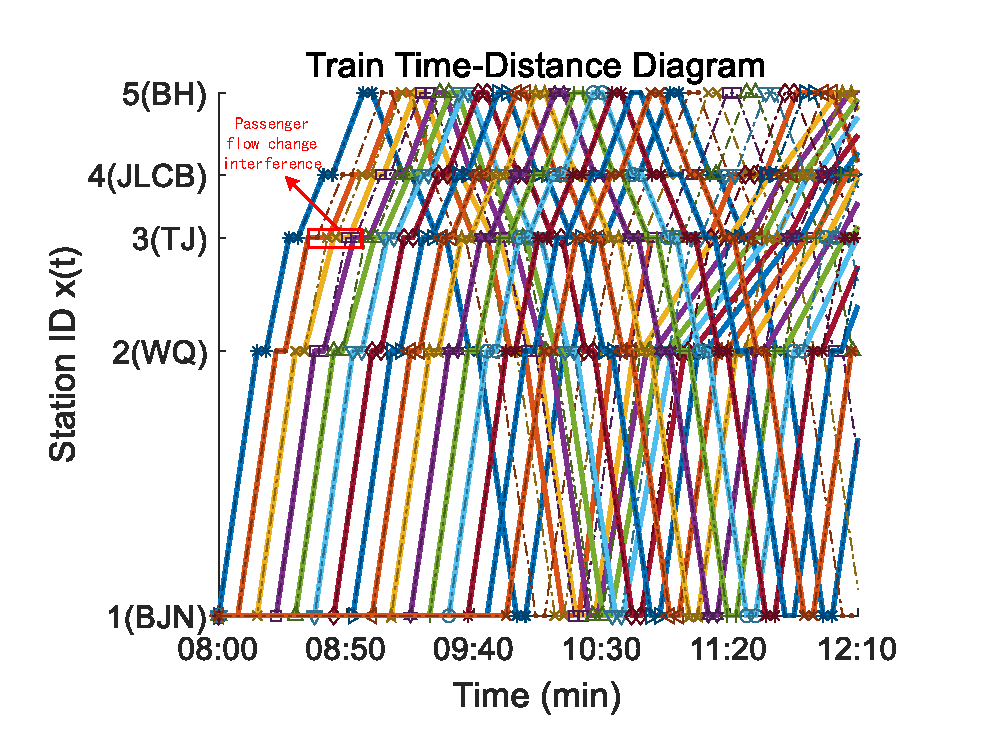
\includegraphics[width=\textwidth]{Img/Ch5/nocontrol.pdf}
	\caption{图定时刻表（虚线）与 FCFS 方法下的实际运行图（实线）}
	\label{fig1:fcfs}
\end{figure}

随后，在相同场景下引入所设计的 IL-MPC 控制器，并开展多轮批次仿真。如图~\ref{fig2:iterative} 所示，在首次迭代中，得益于模型预测控制的前瞻性优化能力，控制器已展现出良好的重调度性能：尽管受客流突变与延误传播影响，列车 2–4 在天津站出现一定程度晚点，但在经过后续四站（JLCBU、BH、JLCBD、TJD）后，其运行时刻逐步恢复至图定状态。图中，“U”表示上行方向，“D”表示折返下行方向。

\begin{figure}
	\centering
	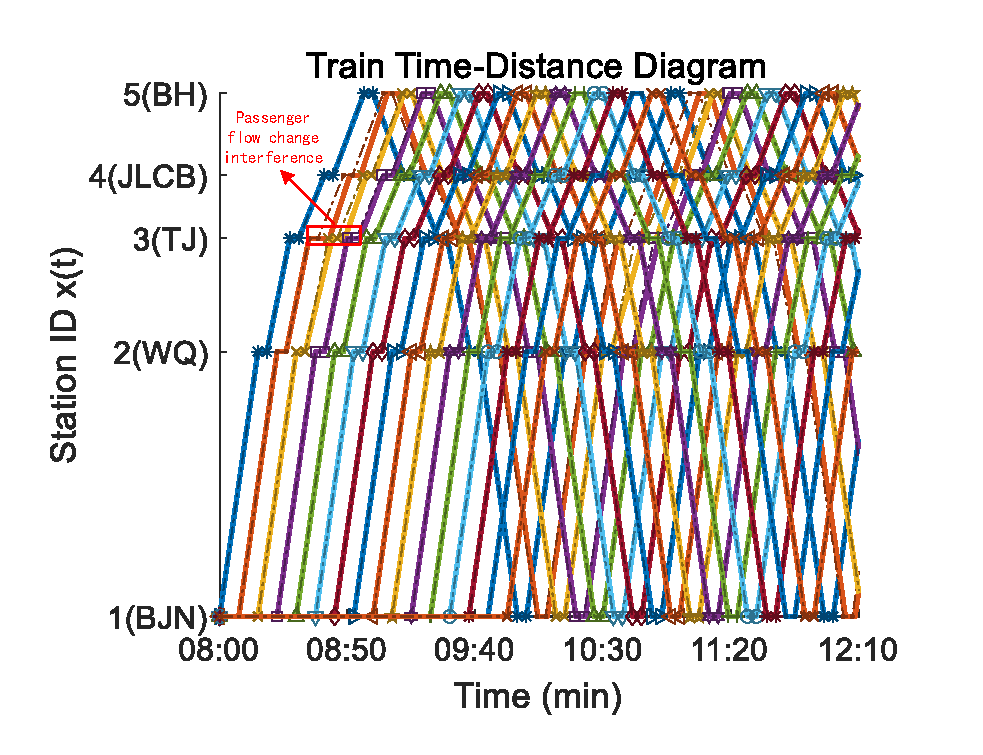
\includegraphics[width=\textwidth]{Img/Ch5/first.pdf}
	\caption{迭代学习模型预测控制方法生成的重调度列车运行图}
	\label{fig2:iterative}
\end{figure}

进一步地，随着迭代次数增加，控制器的学习能力逐步显现。如图~\ref{fig3:total} 所示，系统总延误时间随迭代轮次持续下降。经过 20 轮迭代学习后，重调度效果相较首轮显著提升，表明控制器能够有效利用历史运行信息不断优化当前控制策略。

\begin{figure}
	\centering
	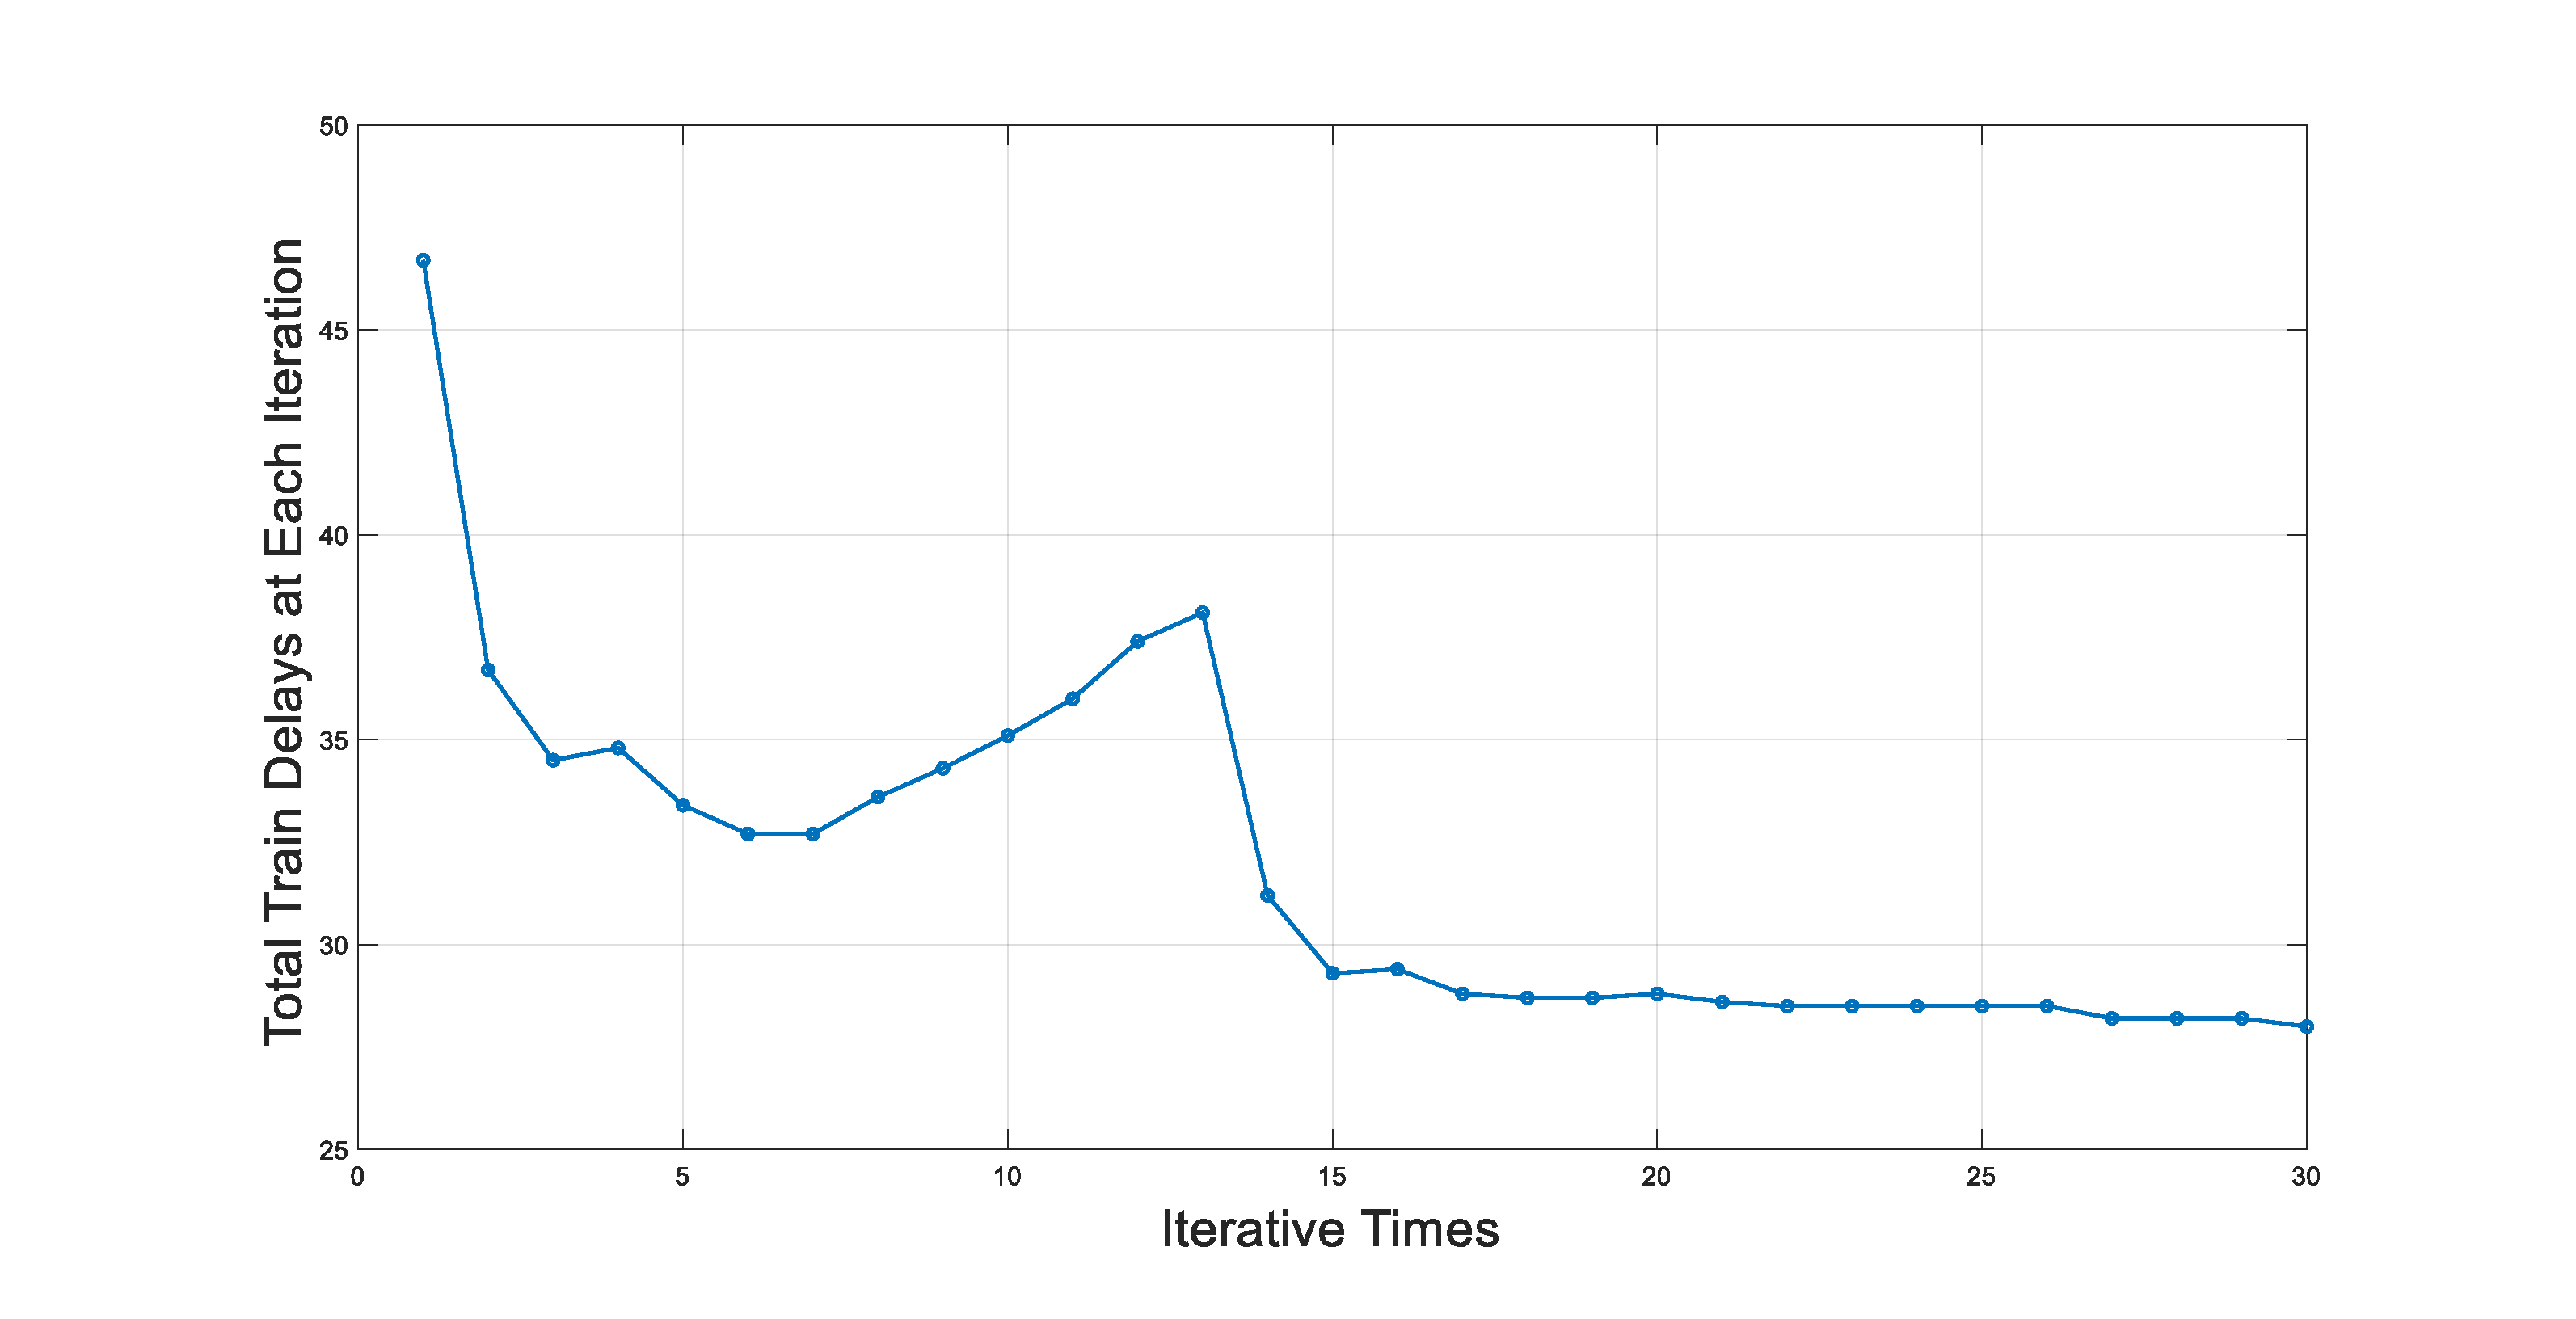
\includegraphics[width=\textwidth]{Img/Ch5/total.pdf}
	\caption{系统总列车延误时间随迭代次数的演化曲线}
	\label{fig3:total}
\end{figure}

为突出对比优势，本文在同一仿真场景下分别实现了传统状态反馈控制器、标准模型预测控制器（MPC）以及混合整数规划（MIP）优化方法。各方法在各车站的累计延误变化如图~\ref{fig4:contrast} 所示。结果表明，所提出的 IL-MPC 控制器在恢复速度、总延误量及抗扰鲁棒性方面均显著优于其他方法。

\begin{figure}
	\centering
	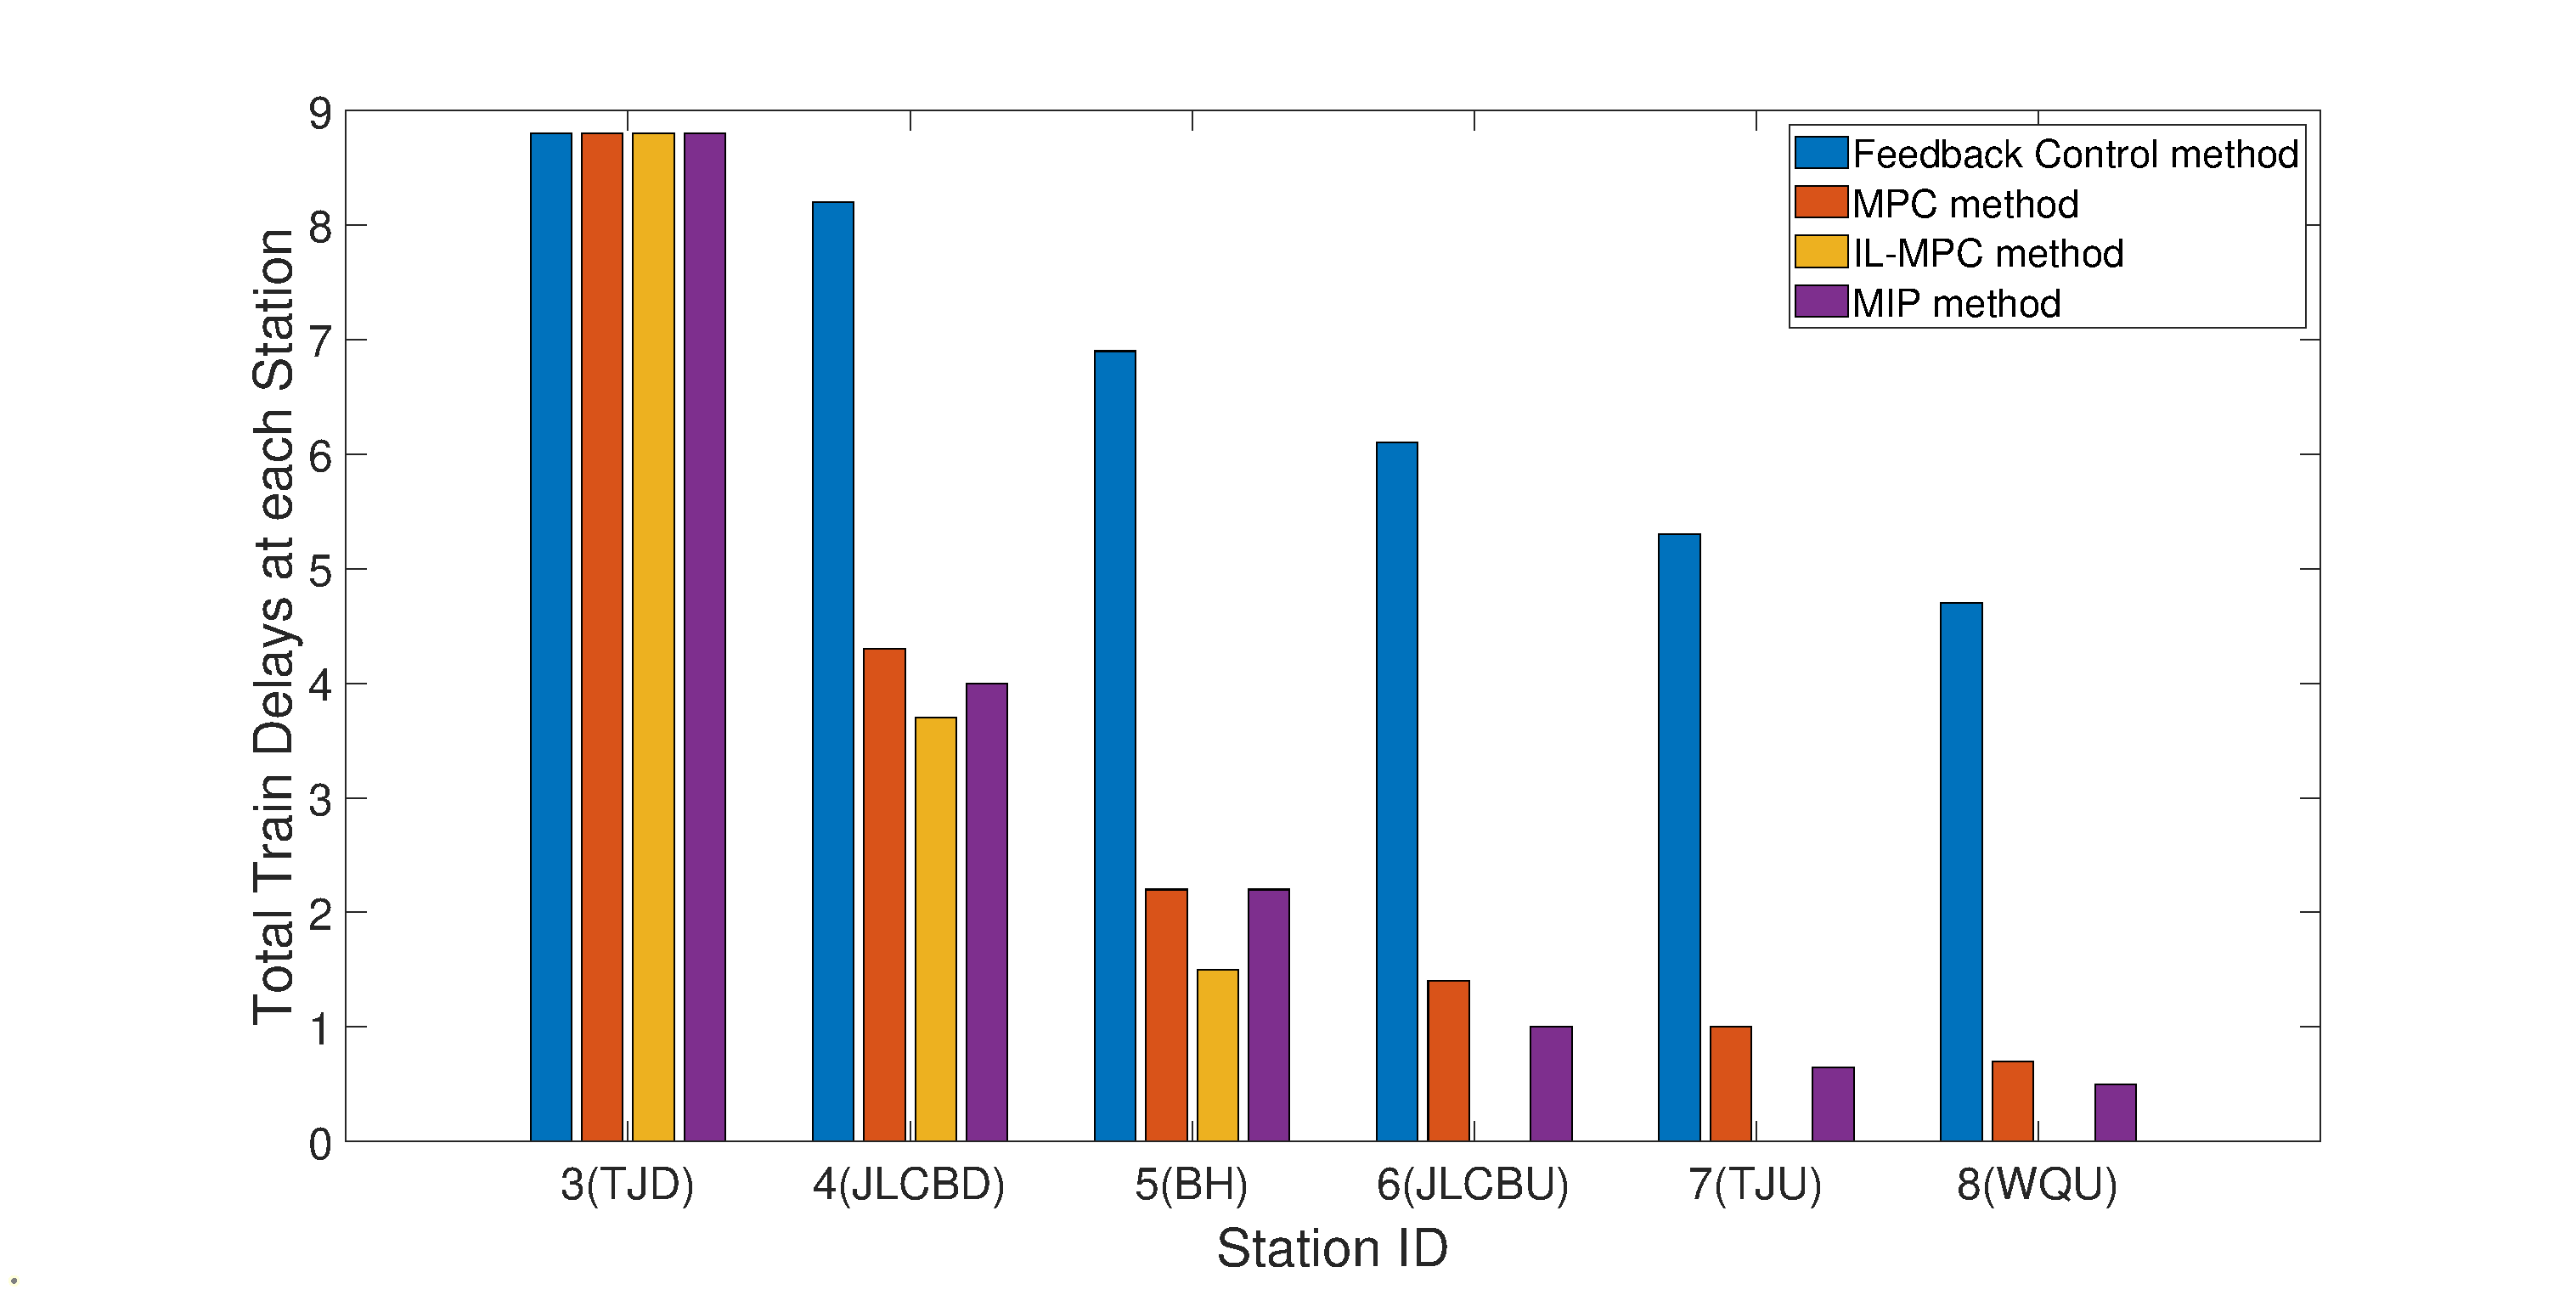
\includegraphics[width=\textwidth]{Img/Ch5/contrast.eps}
	\caption{状态反馈、MPC、IL-MPC 与 MIP 方法在各车站的总延误时间对比}
	\label{fig4:contrast}
\end{figure}

此外，如图~\ref{fig5:time} 所示，IL-MPC 生成的控制量（即发车时刻调整量）在各批次中始终保持在合理范围内，未出现剧烈波动，符合实际运营中对控制动作平滑性的要求。

\begin{figure}
	\centering
	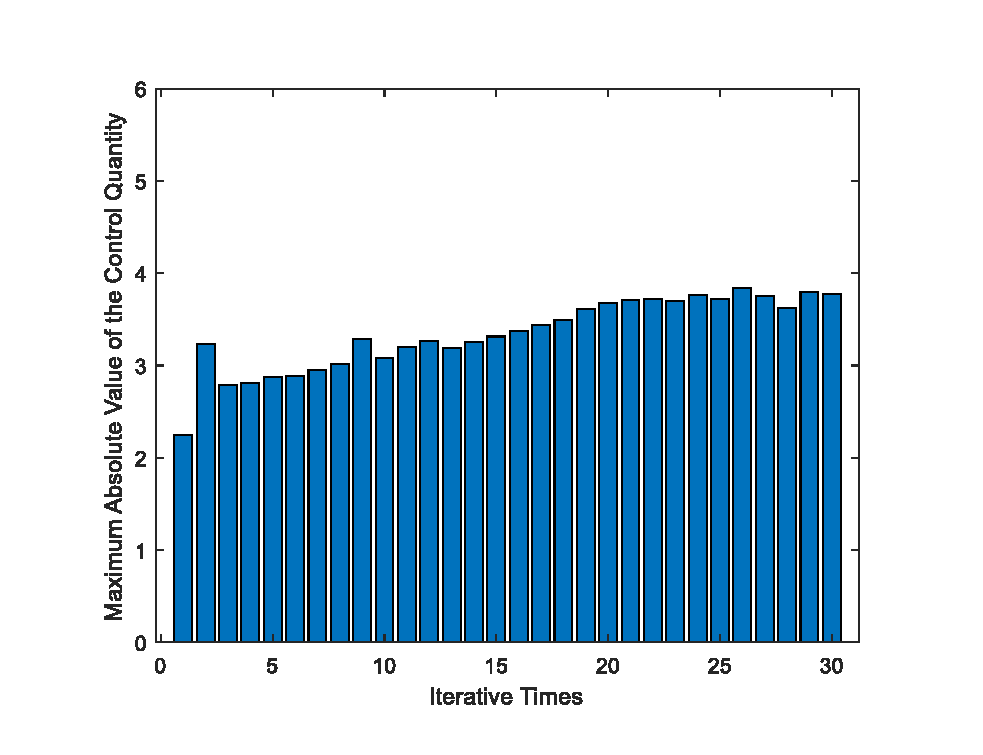
\includegraphics[width=\textwidth]{Img/Ch5/Maxcontrol.pdf}
	\caption{各批次中控制量最大绝对值变化曲线}
	\label{fig5:time}
\end{figure}

最后，如表~\ref{computation time} 所示，IL-MPC 控制器单次迭代的平均计算时间稳定在毫秒级（–0.8 ms），展现出优异的实时性能。这一特性使其在实际工程应用中具备高度可行性，能够快速响应运行环境变化，保障重调度决策的及时性与有效性。

\begin{table}
\centering
\caption{IL-MPC 控制器每批次的平均计算时间}
\begin{tabular}{@{}c@{\hspace{8pt}}c@{\hspace{12pt}}c@{\hspace{8pt}}c@{}}
\hline
\textbf{迭代} & \textbf{平均计算} & \textbf{迭代} & \textbf{平均计算} \\
\textbf{次数} & \textbf{时间 (ms)} & \textbf{次数} & \textbf{时间 (ms)} \\
\hline
1  & 0.7 & 16 & 0.7 \\
2  & 0.8 & 17 & 0.6 \\
3  & 0.6 & 18 & 0.8 \\
4  & 0.5 & 19 & 0.7 \\
5  & 0.6 & 20 & 0.5 \\
6  & 0.8 & 21 & 0.6 \\
7  & 0.7 & 22 & 0.7 \\
8  & 0.7 & 23 & 0.8 \\
9  & 0.5 & 24 & 0.7 \\
10 & 0.7 & 25 & 0.6 \\
11 & 0.6 & 26 & 0.5 \\
12 & 0.8 & 27 & 0.7 \\
13 & 0.7 & 28 & 0.6 \\
14 & 0.5 & 29 & 0.8 \\
15 & 0.6 & 30 & 0.7 \\
\hline
\end{tabular}
\label{computation time}
\end{table}

\section{本章小结}
\label{section6}

本章针对城际高速铁路列车重调度中面临的鲁棒性与运行效率问题，提出了一种融合迭代学习控制与模型预测控制的新型重调度控制器（IL-MPC）。该方法充分利用迭代学习对周期性扰动的补偿能力与模型预测控制对系统动态和约束的显式处理优势，有效提升了系统应对客流突变等外部干扰的能力。

具体而言，首先基于城际高速列车的运行特性，建立了适用于重调度分析的状态空间模型，并进一步构建了批处理形式的动态描述，嵌入了预测时域结构；其次，设计了以时刻表恢复与控制能耗最小化为目标的二次型性能指标，并推导出相应的最优控制律；在此基础上，通过严格的数学分析证明了闭环系统在有界扰动下的收敛性。

为验证所提方法的有效性，本文在京津城际高速铁路仿真平台上开展了系列实验。结果表明：相较于传统的状态反馈控制、标准 MPC 以及混合整数规划（MIP）方法，所提出的 IL-MPC 控制器在抑制延误传播、加快运行秩序恢复方面表现更优；同时，其生成的控制量变化平缓，单次计算耗时稳定在毫秒级，充分满足实际调度对实时性与可操作性的要求。

综上，本章所提出的迭代学习模型预测控制框架为城际高速铁路的高效、鲁棒重调度提供了一种兼具理论严谨性与工程实用性的解决方案。

